\normaltrue
\correctionfalse

%\UPSTIidClasse{11} % 11 sup, 12 spé
%\newcommand{\UPSTIidClasse}{12}

\exer{Mouvement RT  $\star$ \label{C2:08:05}}
\setcounter{question}{0}\UPSTIcompetence[2]{C2-08}
\UPSTIcompetence[2]{C2-09}
\index{Compétence C2-08}
\index{Compétence C2-09}
\index{Torseur cinétique}
\index{Torseur dynamique}
\index{Mécanisme à 1 rotation et 1 translation}
\ifcorrection
\else
\marginnote{\textbf{Pas de corrigé pour cet exercice.}}
\fi

\ifprof
\else
Soit le mécanisme suivant. On a $\vect{AB}=\lambda(t)\vect{i_1}$. De plus :
\begin{itemize}
\item $G_1$ désigne le centre d'inertie de \textbf{1} et $\vect{AG_1}=L_1\vect{i_1}$, on note $m_1$ la masse de \textbf{1} et $\inertie{G_1}{1}=\matinertie{A_1}{B_1}{C_1}{0}{0}{0}{\bas{1}}$; 
\item $G_2=B$ désigne le centre d'inertie de \textbf{2}, on note $m_2$ la masse de \textbf{2} et $\inertie{G_2}{2}=\matinertie{A_2}{B_2}{C_2}{0}{0}{0}{\bas{2}}$.
\end{itemize}
\begin{center}
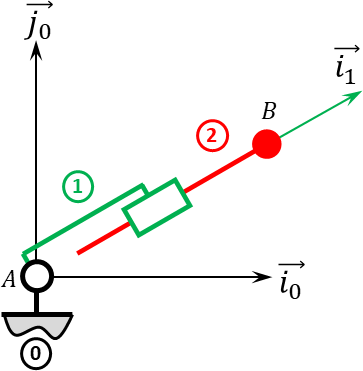
\includegraphics[width=\linewidth]{05_RT_01}
\end{center}

\ifcolle
\else
RESULTAT A VERIFIER!!!!!
Par ailleurs, on donne $\torseurcin{V}{2}{0} =\torseurl{\dot{\theta}(t)\vk{0}}{\dot{\lambda}(t)\vi{1}+\lambda(t)\dot{\theta}(t)\vj{1}}{B}$ et $\vectg{B}{2}{0} =  \left( \ddot{\lambda}(t)-\lambda(t)\dot{\theta}(t)^2\right)\vi{1}  +  \left( \dot{\lambda}(t)\dot{\theta}(t) +\dot{\lambda}(t)\dot{\theta}(t)\right) \vj{1}$.
\fi

\fi



\question{Exprimer le torseur dynamique $\torseurdyn{1}{0}$ en $A$.}

\ifprof
On a $\torseurdyn{1}{0} = \torseurl{\vectrd{1}{0}}{\vectmd{A}{1}{0}}{A}$.

\textbf{Calculons $\vectrd{1}{0}$.}

$\vectrd{1}{0} = m_1 \vectg{G_1}{1}{0}$ $=m_1\dderiv{\vect{AG_1}}{R_0}$
$=m_1\dderiv{L_1\vi{1}}{R_0}$
$=m_1L_1\deriv{\thetap\vj{1}}{R_0}$
$=m_1L_1\left( \thetapp \vj{1} - \thetap^2 \vi{1} \right)$.

\else
\fi

\question{Déterminer $\vectmd{A}{1+2}{0}\cdot \vect{k_0}$}
\ifprof

\else
\fi

\ifcolle
\question{Déterminer les lois de mouvements.}

%\question{Déterminer $\pext{2}{1}{0}$ et $\pext{1}{2}{0}$.}
\else
\fi

\ifprof
\else
\begin{flushright}
\footnotesize{Corrigé  voir \ref{C2:08:05}.}
\end{flushright}%
\fi